\documentclass[12pt, a4paper, oneside]{ctexbook}
\usepackage{amsmath, amsthm, amssymb, bm, graphicx, hyperref, mathrsfs, fancyhdr,adjustbox}

\title{{\Huge{\textbf{计算机控制系统笔记}}}\\
(第一版)}
\author{陈傲}
\date{\today}
\linespread{1.5}
\hypersetup{
	colorlinks=true,
	linkcolor=black
}

\begin{document}

\maketitle

\pagenumbering{roman}
\setcounter{page}{1}

\begin{center}
    \Huge\textbf{前言}
\end{center}~\

这份笔记是基于\textbf{黄大荣}老师课上所讲内容与其PPT整理而成,同时在b站有我本人对应所讲的配套课程,名为《计算机控制系统简明教程》 。这份笔记本来是用markdown书写的,后期我用\LaTeX 加以整理重写,使其更加美观简洁,方便打印。这两种版本我都会在github中开源,但在仓库中我将只提供\LaTeX 版本编译后的PDF文件,而不再markdown版本编译后的PDF文件。

同时由于本人水平一般,能力有限,若在笔记中出现错误内容,恳请大家斧正。

仓库地址:
https://github.com/DylanAo/AHU-AI-Repository。
~\\
\begin{flushright}
    \begin{tabular}{c}
        陈傲\\
        于槐园\\
        \today
    \end{tabular}
\end{flushright}

\newpage
\pagenumbering{Roman}
\setcounter{page}{1}
\tableofcontents
\newpage
\setcounter{page}{1}
\pagenumbering{arabic}

\chapter{离散系统简介}

在本章中,总体是介绍了离散系统相关内容,主要包含以下部分:
\begin{enumerate} 
	\item 离散系统产生(1.1 1.2)
	\item 离散系统使用的数学工具(1.3)
	\item 离散系统的性能指标(1.4)
\end{enumerate}
\newpage 
\section{信号采样与保持}

\subsection{信号的采样}
我们都知道,根据脉冲传递函数的性质,如果一个函数乘上脉冲传递函数,其结果就是函数在0处的值,即为:
$$
f(t)\delta_(t)=f(0)
$$
利用此性质,我们可以得到理想的理想采样序列:
$$
\delta_T(t)=\sum_{n=-\infty}^{\infty}\delta(t-nT)
$$
其中$T$为采样周期,上述式子含义就是每隔一个采样周期有就利用一个脉冲传递函数进行采样。

那么,我现在存在一个连续信号$e(t)$,采样后信号为$e^*(t)$,有:
\begin{equation}
	e^*(t)=e(t)\delta_T(t)=e(t)\sum_{n=-\infty}^{\infty}\delta(t-nT)=\sum_{0}^{\infty}e(nT)\delta(t-nT)
\end{equation}
考虑到现实的物理意义,$e(t)$这个信号在采样前是就是0,所以公式(1.1)的求和是从0开始的。
进行拉普拉斯变换有:
\begin{equation}
	E^*(s)=\sum_{0}^{\infty}e(nT)e^{-nTs}
\end{equation}
公式(1.2)相当于是在作用的幅值延迟$nT$时间,若给你一个连续的信号,让你求采样后的拉氏变换,可以带入公式(1.2)。

我们还知道,傅里叶级数是给你一个任意的函数都能搞成一堆三角函数相加的形式,那么我们采样函数的拉普拉斯变换也能展开成傅里叶级数的形式:
$$
E^*(s)=\frac{1}{T}\sum_{n=-\infty}^{\infty}E(s+jn\omega_s)
$$
即给定一个信号,先用拉普拉斯变换换成$E(s)$,在将$s$换为$s+jn\omega_s$,得到$E(s+jn\omega_s)$,再带入上述式子即可
\subsection{零阶保持器(ZOH)}
零阶保持器就是把输入他的信号保持一个周期$T$(一拍),在这一个周期开始时输入信号为多少,那么在整个周期内输出信号就为开始时刻的输入信号。实际上,这个零阶保持器不就是个门信号,相对于标准的门信号,其宽度为$T$,并且右移了$\frac{T}{2}$
$$
k(t)=1-1(t-T)
$$
$$
G_h(s)=\frac{1-e^{-Ts}}{s}
$$
信号经过零阶保持器可近似看作为在原系统上添加了$\frac{T}{2}$的纯延时环节,所以系统的动态性能指标会变差一些。
\section{脉冲传递函数}

\subsection{定义}
线性离散系统的脉冲传递函数定义为在\textbf{零初始条件下},系统或环节的输出采样函数Z变换和输入采样函数z变换之比。脉冲传递函数只决定于系统本身的结构参数,与输入信号无关,即:
$$
G(z)=\frac{Y(z)}{R(z)}
$$

实际上,这个定义与性质于连续系统中$G(s)$的定义类似,那么我的输出信号就类比与$G(s)$中的输出,可通过类似与连续系统中传递函数的方法求出:
$$
Y(z)=G(z)R(z)
$$

\subsubsection{广义对象脉冲传递函数}
所谓广义对象通常是指保持器环节和被控对象环节串联后所构成的连续时间系统,保持器一般为\textbf{零阶保持器}。
\begin{figure}[htbp]
	\centering
	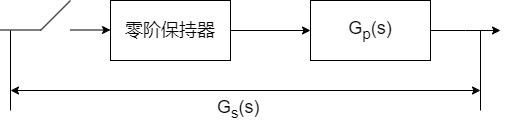
\includegraphics[width=10cm,height=2.6cm]{img/3_5.png}
	\caption{加入零阶保持器的系统框图}
\end{figure}

根据结构框图,我们只需要在被控对象前乘上零阶保持器的传递函数,即:
$$
G(s)=\frac{1-e^{-Ts}}{s}G_p(s)
$$
然后对上述$G(s)$进行z变换,即可求出广义对象脉冲传递函数:
\begin{equation}
	G(z)=\frac{z-1}{z}\mathcal Z[\frac{G_p(s)}{s}] = 1-z^{-1}\mathcal Z[\frac{G_p(s)}{s}]
\end{equation}
公式(1.3)是非常重要的公式,在后续章节和题目中我们会经常看见它,请牢记!
\subsection{给定框图求脉冲传递函数}
\subsubsection{开环脉冲传递函数}
\begin{figure}[htbp]
	\centering
	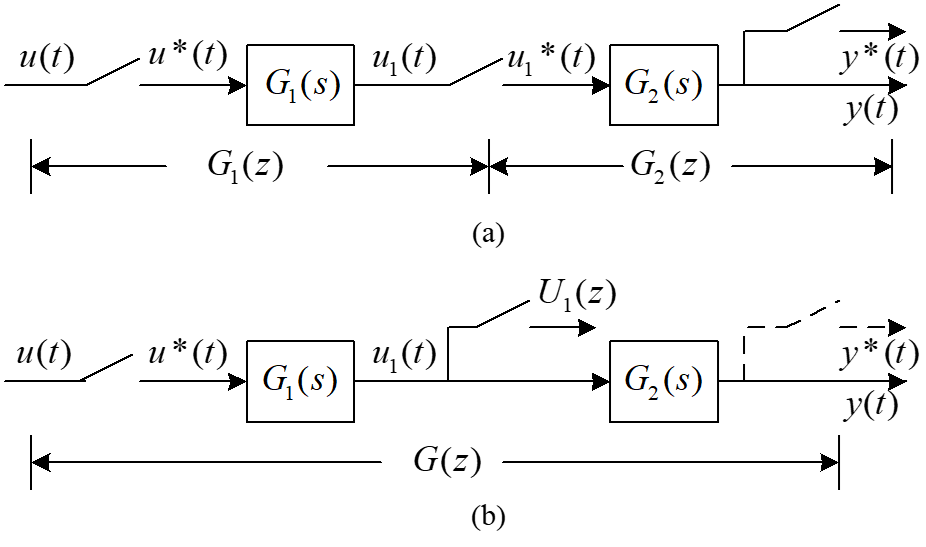
\includegraphics[width=10cm,height=5.47cm]{img/1_1.png}
	\caption{开环脉冲传递函数框图}
\end{figure}

在图1.2-a中,两个串联环节之间存在采样开关,得到的脉冲传递函数为:
$$
G(z)=G_1(z)G_2(z)
$$

在图1.2-b中,两个串联环节之间不存在采样开关,得到的脉冲传递函数为:
$$
G(z)=G_1G_2(z)
$$

值得注意的是,$G_1(z)G_2(z)$是$G_1(s)$与$G_2(s)$\textbf{分别做z变换然后相乘的结果},而$G_1G_2(z)$是$G_1(s)$与$G_2(s)$\textbf{先相乘,得到的乘积再做z变换},而在通常情况下$G_1(z)G_2(z)\neq G_1G_2(z)$。

针对并联环节而言,只需要将并联的两个关节相加减即可。

实际上并不是所有的环节都能求出$G(z)$的,若是出现在信号输入处没有采样环节,那么就求不出$G(z)$。最后是用$Y(z)$来表示,同样的,这要遵循上述的基本运算规则:
\begin{figure}[htbp]
	\centering
	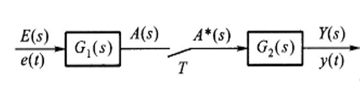
\includegraphics[width=10.8cm,height=2.64cm]{img/1_2.png}
	\caption{开环脉冲传递函数框图2}
\end{figure}

例如图1.3可表示为:(注意中间有采样环节)
$$
Y(z)=G_1E(s)G_2(s)
$$
\subsubsection{闭环脉冲传递函数}
闭环脉冲传递函数实际上是在开环基础上求出的,即:
$$
\mbox{闭环传递函数}=\frac{\mbox{前向通道所有独立环节的Z变换乘积}}{1+\mbox{闭环回路中所有独立环节的Z变换乘积}}
$$

所谓独立环节,指的是两个相邻采样开关之间的环节。特别注意,若是闭环系统的输入信号未被采样,则整个系统的闭环脉冲传递函数写不出来,我们按照上述公式求出的是$Y(z)$而非$\Phi(z)$。

\begin{figure}[htbp]
	\centering
	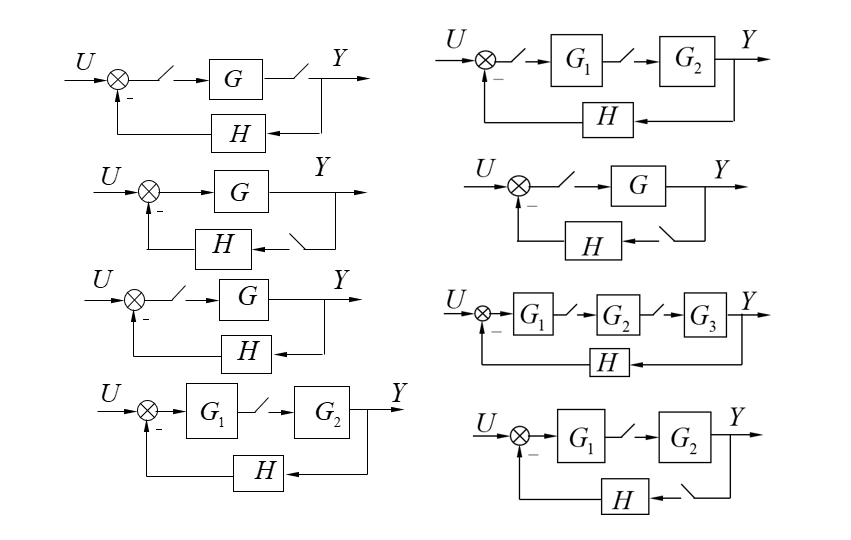
\includegraphics[width=10cm,height=6cm]{img/1_3.png}
	\caption{闭环脉冲传递函数框图}
\end{figure}

值得注意的是,由于分母中要求闭环\textbf{回路}中所有独立环节的Z变换乘积,要注意$H$与$G_1$之间其实是连着的。
这里有个结论,如果H的两侧都有采样开关,那么H是一个单独环节,要\textbf{单独乘}(如图1.4左上角);若H两侧不全有采样开关,那么H就是不是一个单独环节,要\textbf{乘到一起}(如图1.4左下角),这个结论本质上仍然是判断是不是独立环节。
上图左上角系统传递函数为:
$$
\Phi(z)=\frac{G_1(z)}{1+G_1H(z)}
$$
上图左下角系统传递函数为(注意输入信号无采样):
$$
Y(z)=\frac{G_1U(z)G_2(z)}{1+G_1G_2H(z)}
$$
正常题目中,一般给的是形如$G_1(s)$的$s$变换,所以一定要注意$G_1(z)G_2(z)$
与$G_1G_2(z)$的区别
\section{Z变换与逆Z变换}
采样是物理过程,是连续系统转化为离散系统的过程.离散系统是用差分方程描述的,在数学上可以利用Z变换进行求解等操作。

实际上给定$G(s)$需要先变为$g(t)$,然后进行\textbf{采样}得到$g^*(t)$,最后进行z变换得到$G(z)$
只不过s变换与z变换直接存在一定联系,在知道采样周期后可以利用这个联系直接从s变到z,而不用先s域变时域,采样得到离散时域然后再变z域。具体的联系是我们这节要讲的内容。

\subsection{Z变换}
z变换本质上是将采样后的拉式变换中$e^{-Ts}$代换为$z$,即:
$$
z=e^{-Ts}\\
E(z)=\sum_{0}^{\infty}e(nT)z^{-n}
$$
\subsubsection{部分分式展开法}
\begin{figure}[htbp]
	\centering
	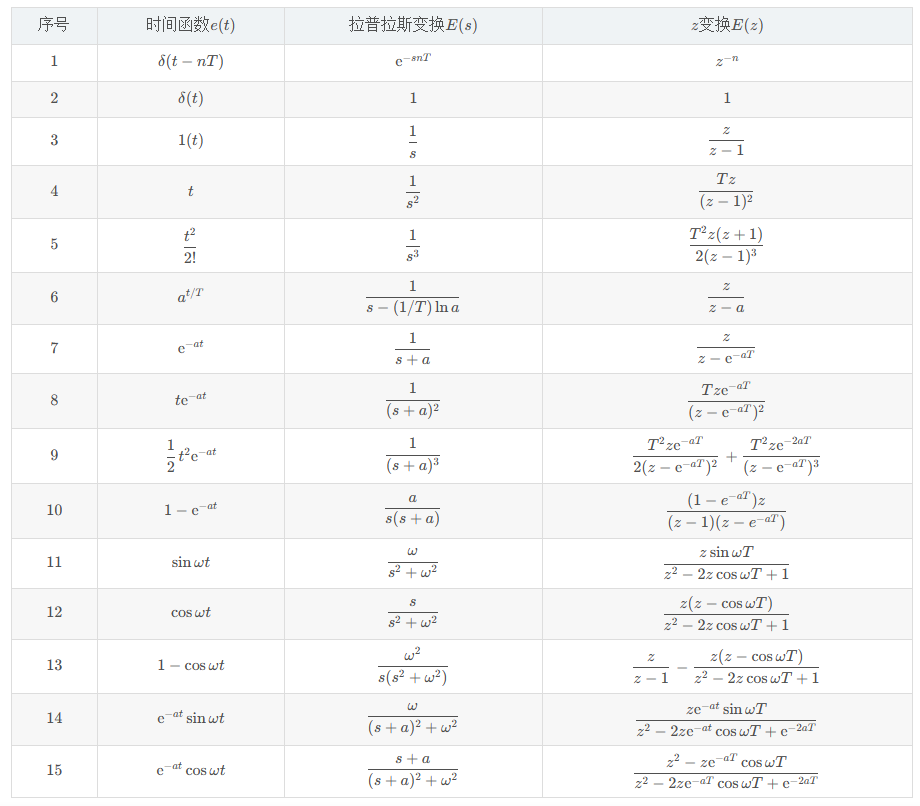
\includegraphics[width=16cm,height=11cm]{img/2_1.png}
	\caption{常见的变换对表}
\end{figure}

最常见情况是先进行部分分式展开,然后利用上表查表得到的变换后的结果。
\subsubsection{留数法}
留数从数学上来说定义如下:
$$
Res[f(z),z_0]=\frac{1}{(n-1)!}lim_{z\rightarrow z_0}[(z-z_0)^nf(z)]^{n-1}
$$
其中,n为极点级数。
对此,我们不难发现,要是1级极点,那么留数求法就会变成异常简单。
$$
Res[f(z),z_0]=lim_{z\rightarrow z_0}(z-z_0)f(z)
$$
而且,通常情况下,$(z-z_0)$是可以和$f(z)$分母上多项式约掉的,会变得更简单。

用留数法求z变换,就用下述公式:
$$
F(z)=\sum_{i=1}^nRes[F(s)\frac{1}{1-e^{sT}z^{-1}}]\bigg|_{s=s_i}
$$
也就是说,求$F(z)$那么就将$F(s)$乘上$\frac{1}{1-e^{sT}z^{-1}}$,然后挨个极点求留数(每个极点都要跟着这个东西)就行了
值得注意的是,在遇到二阶以上极点要进行求导运算,这里求导是\textbf{对s求导},那么\textbf{不要忘记$\frac{1}{1-e^{sT}z^{-1}}$也要参与求导运算}。

\subsection{逆Z变换}
\subsubsection{多项式展开与系数快速确定}
我们以下述式子为例:
\begin{equation}
	\frac{1}{(z^2+1)(z+1)} = \frac{Az+B}{z^2+1}+\frac{C}{z+1}
\end{equation}
拆分前是分母是多项式相乘的样子,拆分后就是把分母单独提出来作为一个式子,而分子的系数为次数分母的最高系数减1一直到0(常数)。

若是:
\begin{equation}
	\frac{1}{(z^2+1)^2} = \frac{Az+B}{(z^2+1)^2}+\frac{Cz+D}{z^2+1}
\end{equation}
若分母中的括号为n次,那么拆开后分母从n至n-1次都要写出来,分子的次数对应上一条规则来写。

对于快速计算系数,我们以公式(1.4)为例,其原理如下:
若想求$z-1$对应系数,则有左右同乘$z-1$:
$$
\frac{1}{(z^2+1)} = \frac{Az+B}{z^2+1}(z-1)+C
$$
然后将$z_0=1$带入有(就是上述同乘的式子等于0的解):
$$
\frac{1}{(z^2+1)}\bigg|_{z_0=1} = \frac{Az+B}{z^2+1}(z-1)\bigg|_{z_0=1}+C\\
\frac{1}{(z^2+1)}\bigg|_{z_0=1}=C\\
$$
$$
C=2
$$
值得注意的是,我们在求C的值时候,C前面是没有Z的,也就是说实际上可简写为(示例,不一定与上面的一致):
$$
F(z)(z-2)\bigg|_{z_0=2}=C
$$
而不是:
\begin{equation}
	F(z)(z-2)\bigg|_{z_0=2}=zC
\end{equation}

$$
\frac{F(z)(z-2)}{z}\bigg|_{z_0=2}=C
$$
若是遇到公式(1.6)情况,一定要注意z的值,\textbf{左侧带入$z_0$后求解的其实是$z_0C$而非C}。

假设我们遇到公式(1.5)类似的分母带系数的情况:
$$
\frac{1}{(z+1)^2(z+3)} = \frac{A}{(z+1)^2}+\frac{B}{z+1}+\frac{C}{z+3}
$$
那么就需要求导,对于最高阶对应的系数(A)实际上就是:
$$
\frac{1}{(z+1)^2(z+3)}(z+1)^2= A+B(z+1)+\frac{C}{z+3}(z+1)^2\bigg|_{Z_0=-1}\\
\frac{1}{(z+3)}\bigg|_{Z_0=-1}= A
$$
而剩下的系数(B)就分别对应求导:
$$
\frac{d}{dz}[\frac{1}{(z+1)^2(z+3)}(z+1)^2]= \frac{d}{dz}[A+B(z+1)+\frac{C}{z+3}(z+1)]
$$
$$
\frac{d}{dz}[\frac{1}{(z+3)}]\bigg|_{Z_0=-1}= B+\frac{C}{z+3}2(z+1)\bigg|_{Z_0=-1}
$$
$$
\frac{d}{dz}[\frac{1}{(z+3)}]\bigg|_{Z_0=-1}= B
$$
而其他的系数(C)正常求即可

对于快速求系数的结论就是:
\begin{enumerate} 
	\item 将展开后的分母乘到展开前的式子,带入极点就是对应分母的分子系数。
	\item 遇到分母外括号带系数的,最高阶按照1正常算,剩下的依次求导计算。
\end{enumerate}

\subsubsection{部分分式展开法中的计算要点}

\noindent 在此处,常见的换对还有:
$$\frac{z}{z-a}\leftrightarrow a^k$$
同时,最主要是用到Z变换的平移性质性质:
$$
f(t-nT) \leftrightarrow z^{-n}F(z) \quad \mbox{右移n}
$$
$$
f(t+nT) \leftrightarrow z^{n}F(z) - \sum_{j=0}^{n-1}z^{n-j}f(j) \quad \mbox{左移n}
$$
我们以此为例:
$$
F(z)=\frac{10z}{(z-1)(z-0.2)}
$$
我们可以直接展开,即为:
$$
F(z)=\frac{12.5}{z-1}-\frac{2.5}{z-0.2}
$$
我们想要按照变换对进行逆变换,很明显分子少z,那我们就乘z:
$$
zF(z)=\frac{12.5z}{z-1}-\frac{2.5z}{z-0.2}\leftrightarrow12.5(1)^k-2.5(0.2)^k
$$
注意,我们求出来的是$zF(z)$的逆变换,而不是$F(z)$逆变换,前者右移一个即为后者:
$$
F(z)=12.5(1)^{k-1}-2.5(0.2)^{k-1}=12.5-12.5(0.2)^k
$$
但是此题仍然有第二种解法:


\begin{equation}
	\begin{aligned}
	\frac{F(z)}{z}&=\frac{10}{(z-1)(z-0.2)}\\ \notag
	&=\frac{12.5}{z-1}-\frac{12.5}{z-0.2}\\ \notag
	\end{aligned}
\end{equation}
$$
F(z)=\frac{12.5z}{z-1}-\frac{12.5z}{z-0.2}\leftrightarrow 12.5-12.5(0.2)^k
$$

值得注意的是,右移是不需要进行额外的加减的,只需要将$k-n$带入即可,如果是左移,那么就需要减去移走的值了:
$$
\frac{F(z)}{z}=\frac{2z}{z-1}-\frac{2z}{z-0.5}\leftrightarrow2(1)^k-2(0.5)^k
$$
$$
F(z)\leftrightarrow2(1)^{k+1}-2(0.5)^{k+1}-2+2=2-0.5^k
$$
\subsubsection{留数法}

\noindent 而用留数法求$F(kT)$也比较简单:
$$
F(kT)=\sum_{i=1}^nRes[F(z)z^{k-1}]\bigg|_{z=z_i}
$$
求$F(kT)$那么就将$F(z)$乘上$z^{k-1}$,然后对每个极点求留数(每个极点也要跟着这个东西)
同样的,对应高阶级点进行求导运算时,也要\textbf{注意$z^{k-1}$也是参与求导运算}。
习惯上,我们将$F(kT)$简写为$F(k)$。

\section{离散系统的性能分析} 
\subsection{s平面到z平面} 
若在s平面中,一个点的坐标为$s=\sigma+\omega j$,映射到z平面后用极坐标表示,即$|z|$为映射后点的模值,$\theta$为映射后角度:
$$
z=e^{Ts}\\
|z|=e^{T\sigma}\qquad \theta=T\omega
$$
注意,上述式子中$\omega$是s平面上点的y坐标,若是题目给你采样频率$\omega_c$,那么实际上给的是$T$,即为$T=\frac{2\pi}{\omega}$。

在s平面中,在特征方程的根在平面左侧为系统稳定,那么根据上述式子我们发现,z平面实际上就是把s平面中竖线掰弯,形成一个圆,那么y轴掰弯后形成的是单位圆,即特征方程的根都在单位圆内,则系统稳定。
\subsection{稳定判据}
由上述变换关系,我们得出结论,线性离散控制系统稳定的充要条件是:
闭环系统特征方程的所有根的模$|z_i|<1$,即闭环脉冲传递函数的极点(特征方程的根)均位于z平面的单位圆内。

众所周知,求出所有的根是十分痛苦且很多情况是不可能的,那么就和连续系统一样,有一些判据来判断系统是不是稳定的。
\subsubsection{w变换及w域的劳斯稳定判据} 
劳斯判据是在自动控制原理提出的,本质上他是在s平面上判断方程的根是否在左半轴。而z变换后,是将是s平面上的点对应到z平面上一个个圆上了,稳定判据从特征方程的根都在左半平面变为都在单位圆内。

\noindent 那么,我能不能想办法通过某种对应方式将z平面上点对应到类似的s平面上,然后通过劳斯判据进行判断呢?

\noindent 实际上,这种对应关系就是我们的w变换:
$$
w变换(双线性变换)\quad
\left\{  
\begin{array}{lr}  
	z=\frac{1+w}{1-w}   \\  
	w=\frac{z-1}{z+1}  
\end{array}  
\right.  
$$
同时,对于双线性变换还可以有好多组,你可以任选一组你喜欢的进行变换:
$$
\left\{  
\begin{array}{lr}  
	z=\frac{w+1}{w-1}   \\  
	w=\frac{z+1}{z-1}  
\end{array}  
\right.\quad
\left\{  
\begin{array}{lr}  
	z=\frac{1+\frac{T}{2}w}{1-\frac{T}{2}w}   \\  
	w=\frac{2}{T}\frac{z-1}{z+1}  
\end{array}  
\right.
\\
$$

将在z平面的式子通过w变换变为w变换后,就可利用劳斯判据判断稳定性了,而且判断过程,结论与s平面上的劳斯判据如出一辙。实际上,当采样周期无限小的时候,w平面近似为s平面。

假设我们有一特征方程为:$z^2-z+0.632=0$,
那么我们利用最后一组的双线性变换,可以得到:
$$0.658w^2+0.368w+0.632=0$$
然后利用劳斯判据,那么劳斯表如下所示:
\begin{figure}[htbp]
	\centering
	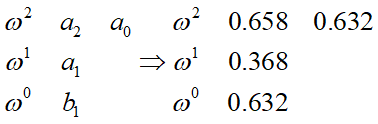
\includegraphics[width=7.56cm,height=2.48cm]{img/3_1.png}
	\caption{例题对应劳斯表}
\end{figure}

\subsubsection{二阶系统z域直接判定法} 
\noindent 我们有如下二阶闭环系统:
$$
W(z)=z^2+a_1z+a_0
$$
满足全部以下条件,则系统稳定:
1. $|W(0)|=a_0=1$
2. $W(1)>0$
3. $W(-1)>0$

\subsubsection{z域中朱利稳定判据} 
我们将特征方程记为$D(z)$,$D(z)$若是稳定的,那么需要\textbf{满足以下全部}条件,在此处我们以$D(z)=-39+119z-117z^2+45z^3$为例:

\noindent \textbf{条件一:} $D(1)>0$,$D(1)=8>0$

\noindent \textbf{条件二:} $\left\{  
\begin{array}{lr}  
	D(-1) > 0 \quad \mbox{最高次项幂为偶数}   \\  
	D(-1) < 0 \quad \mbox{最高次项幂为奇数}
\end{array}  
\right.
$

\noindent 此例题中$D(-1)=-320<0 \quad \mbox{最高次幂系数是3为奇数}$

\noindent 需要列出朱利表,然后再进行条件判断,这个例题的朱利表如下:
\begin{table}[!ht]
	\centering
	\caption{朱利表}
	\begin{tabular}{|l|l|l|l|l|}
		\hline
		~ & $z^{0}$ & $z^{1}$ & $z^{2}$ & $z^{3}$ \\ \hline
		1 & -39 & 119 & -117 & 45 \\ \hline
		2 & 45 & -117 & 119 & -39 \\ \hline
		3 & -504 & 624 & -792 & ~ \\ \hline
		4 & -792 & 624 & -504 & ~ \\ \hline
	\end{tabular}
\end{table}

\noindent 求朱利表的步骤如下:
\begin{enumerate} 
	\item 将$D(z)$升序排列,将其系数写在第一行。
	\item 将第一行反过来,写在第二行。
	\item 取第一行第二列的值,取最右侧第一行第二行值,放到一起,求行列式,放到第三行第一个。行列式最左侧的数不动,从右侧挪一个位置,取右侧倒数第二第一行第二行值,求行列式,依此类推,求出第三行。
	\item 将第三行反过来,写在第四号。
	\item 第五行第六行重复步骤3、4,直到最后一行剩下三个数为止。
\end{enumerate}

\noindent 此例子中,第四行已经只剩下三个数了,所有只算到第四号行可

\noindent \textbf{条件三:}
\begin{enumerate} 
	\item 仅看第一列,对第一列的数取模(绝对值)。
	\item \textbf{第一行的数要小于第二行}。
	\item 从第三行起,每两行为一组,不可以有交集,前一行的要大于后一行,即\textbf{第三行的数要大于第四行,第五行的数要大于第六行},依次类推都是大于。
\end{enumerate}

\noindent 在此例子中,第三行的绝对值没有大于第四号的绝对值,所以系统不稳定。
\subsubsection{修尔-科恩稳定判据} 
已知特征方程为$1+G(z)=0$,我们取特征方程的分子为:
$$W(z)=a_nz^n+a_{n-1}z^{n-1}+···+a_1z^1+a_0=0$$
那么可以根据下表写出一些行列式:
\begin{figure}[htbp]
	\centering
	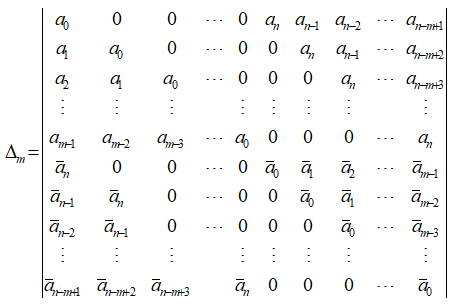
\includegraphics[width=9cm,height=6cm]{img/3_4.png}
	\caption{修尔-科恩稳定判据}
\end{figure}

我们令$m=1,2,···,n$,$n$为特征方程阶数,$\bar{a_n}$为$a_n$的共轭复数。
实际上,我们的$\Delta_m$是$2m\times 2m$的行列式,我们可以写出n个,即$\Delta_n \Delta_{m-1},···,\Delta_1$。

\noindent 这些$\Delta$改变符号的次数就是稳定根的数目,即系统稳定,那么改变符号的次数就是特征方程的阶数
$$
\left\{  
\begin{array}{lr}  
	\Delta_m > 0 \quad \mbox{m为偶数 }  \\  
	\Delta_m < 0 \quad \mbox{m为奇数}
\end{array}  
\right.
$$
\subsection{稳态误差}
\subsubsection{求解稳态误差的一般方法}
\begin{figure}[htbp]
	\centering
	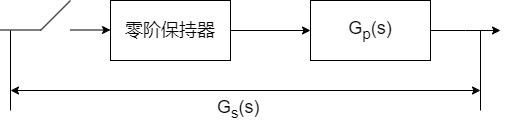
\includegraphics[width=10cm,height=2.6cm]{img/3_5.png}
	\caption{加入零阶段保持器的系统框图}
\end{figure}

根据所示系统环节,求\textbf{开环}脉冲传递函数(注意采样开关的设置):
$$
GH(z)=\frac{1}{(z-1)^v}GH_0(z)\\
\lim_{z\to 1} GH_0(z)=k
$$
其中,上述式子中的$v$为系统的型数。

\noindent 那么,计算稳态误差步骤如下:

\noindent 1. 判定稳定性

\noindent 2. 求误差脉冲传递函数
$$
\phi_e(z)=\frac{E(z)}{R(z)}=\frac{1}{1+GH(z)}
$$

\noindent 3. 利用终值定理求$e(\infty)$
$$
e(\infty)=\lim_{z \to 1}(z-1)\phi_e(z)R(z)=\lim_{z \to 1}(z-1)R(z)\frac{1}{1+GH(z)}
$$
\subsubsection{静态误差系数法} 
与连续系统相同,在离散系统中我们也可以得到静态误差系数来求解稳态误差,在上面我们知道了系统的型数为\textbf{开环脉冲传递函数}中的$v$:
$$
GH(z)=\frac{1}{(z-1)^v}GH_0(z)\\
$$
那么类比连续系统,我们就有:
\begin{equation}
	\begin{aligned}
		\mbox{静态位置误差系数} \quad k_p&=\lim_{z\to 1}GH(z)\\ \notag
		\mbox{静态速度误差系数} \quad k_v&=\frac{1}{T}\lim_{z\to 1}(z-1)GH(z)\\ \notag
		\mbox{静态加速度误差系数} \quad k_p&=\frac{1}{T^2}\lim_{z\to 1}(z-1)^2GH(z)\\ \notag
	\end{aligned}
\end{equation}

\begin{figure}[htbp]
	\centering
	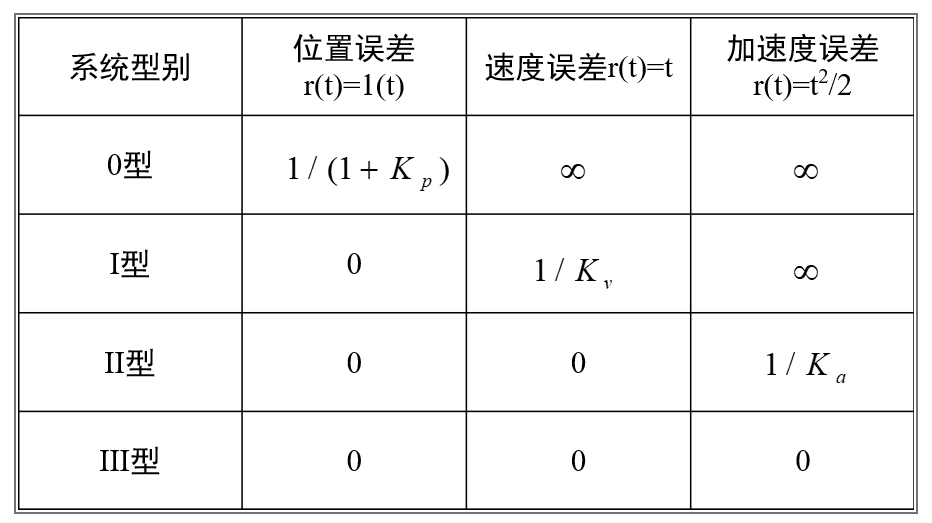
\includegraphics[width=9.32cm,height=5.23cm]{img/4_2.png}
\end{figure}
\subsection{根轨迹法} 
利用根轨迹法可以分析系统的动态性能,在z平面中画根轨迹与在s平面中画根轨迹方法\textbf{完全相同},只不过在s平面上,我们说在左半轴内的规矩是稳定的,而在z平面上,是在单位圆内是稳定的。也就是说,按照自动控制原理中根轨迹画法画出根轨迹,然后再画一个单位圆,在圆内稳定,圆上临界稳定,圆外不稳定。

\subsection{极点分布对动态性能影响} 
\begin{enumerate} 
	\item 闭环极点最好分布在z平面单位圆的右半部,最为理想的是分布在靠近原点的地方,由于这时$|z_j|$值较小,所以相应的瞬态过程较快,即离散系统对输入具有快速响应的性能。
	\item 和连续系统中相同,离散系统中也有主导极点,统响应主要由这一对主导极点决定,其他极点在分析时可忽略不计。主导极点是最靠见单位圆的极点。
\end{enumerate}
\newpage
\chapter{设计离散系统}
在本章中我们主要介绍如何设计离散系统,使其满足我们的需求,主要内容如下:
\begin{enumerate} 
	\item 间接设计法(2.1)
	\item 直接设计法(2.2)
	\item 状态空间设计法(2.3)
\end{enumerate}
\newpage
\section{间接设计法}
将计算机控制系统近似地看成是一个连续变化的模拟系统,用模拟系统的理论和方法进行分析和设计,得到模拟控制器,然后再将模拟控制器进行离散化,得到数字控制器,这种设计方法叫间接设计法,其中典型的算法为PID算法。

这里我们只是提到对控制器进行离散化,那么对控制对象用不用离散化?
答案是不用,因为我们的控制对象前面会接入D/A转换器,他输入的是连续量而非离散量,如下图所示:
\begin{figure}[htbp]
	\centering
	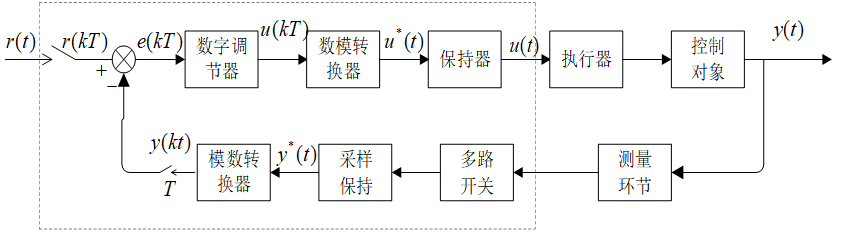
\includegraphics[width=12cm,height=3.2cm]{img/5_5.png}
	\caption{一般控制流程图}
\end{figure}

\subsection{常用的离散化方法}
对于模拟控制器,我们要把他进行离散化,能否直接采样不就离散化?实际上,这是一种离散化办法(脉冲响应不变法),这里还有其他的离散化办法:

前向差分变换(实际一般不用)
$$
s=\frac{z-1}{T}
$$

后向差分变换(常用)
$$
s=\frac{1-z^{-1}}{T}
$$

双线性变化法
$$
s=\frac{2}{T}\frac{z-1}{z+1}
$$

脉冲响应不变法

\noindent 这种实际上就是采样然后z变换过程,给采样周期直接做z变换即可得到。
所谓脉冲响应不变法就是将连续滤波器离散得到离散滤波器后,它的脉冲响应与连续滤波器的脉冲响应在各采样时刻的值是相等的。

阶跃响应不变法

\noindent 有点类似于加上零阶保持器然后z变换的过程,前面带零阶保持器的z变换怎么求,这里就怎么求。
所谓阶跃响应不变法就是将连续滤波器离散后得到的离散滤波器,保证其阶跃响应与原连续滤波器的阶跃响应在各采样时刻的值是相等的。

$$
G(z)=\frac{z-1}{z}\mathcal Z[\frac{G_p(s)}{s}]
$$

零极点匹配法
\begin{figure}[htbp]
	\centering
	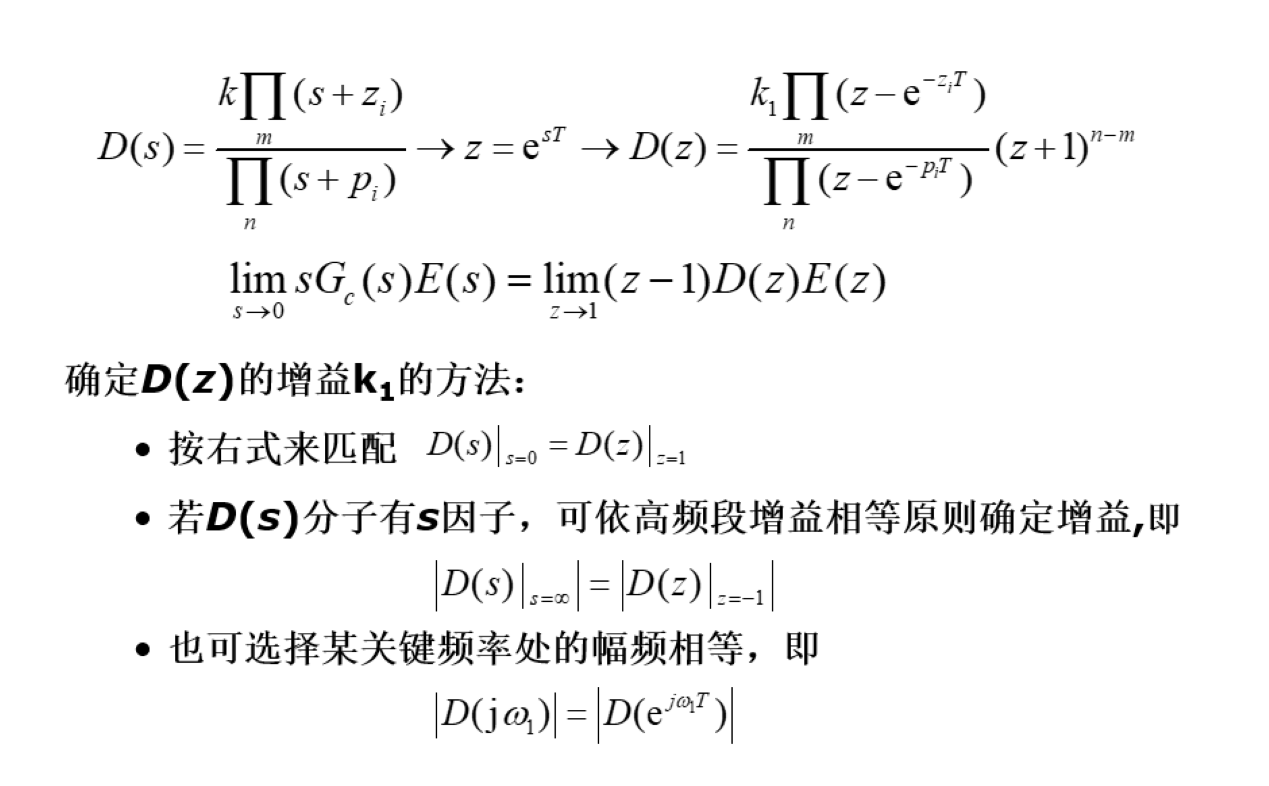
\includegraphics[width=12.6cm,height=7.89cm]{img/5_1.png}
\end{figure}

\textbf{小结}

1. 后向差分与双线性变换较为常用

2. 在采样周期$T$较小时,各种变换方法区别不大

3. 零极点匹配法效果最好,但比较复杂,在要求较高时使用
\subsection{数字PID控制器} 
数字式PID是在模拟型PID上离散化过来的,那么对于模拟型PID我们有以下式子:
$$
u(t)=K_p[e(t)+\frac{1}{T_I}\int_0^te(t)d(t)+T_D\frac{de(t)}{dt}]
$$
实际上对于上述所有的离散方法,这里都能用,但是一般在工程上我们只用后向差分这一种方法,这里都是基于后向差分得到的,具体推导过程如下:

1. 对于时间$t$,则变为$t=KT$,通常我们省略$T$不写,只留$K$

2. 比例环节不变,积分环节就变成了长度为采样周期,高度为采样值的长方形面积加在一起(就是微元法),即:$\int e(t)dt=T\sum_{j=0}^ke(jT)$

3. 微分环节就变成了后向差分,即:$\frac{de(t)}{dt}=\frac{e(kT)-e[(k-1)T]}{T}$

\noindent 我们将上述式子替换过去,就得到了位置式PID控制的方程。
\subsubsection{位置式PID控制} 
$$
u(k)=K_p[e(k)+\frac{T}{T_1}\sum^{k}_{j=0}e(j)+\frac{T_D}{T}[e(k)-e(k-1)]]\\
=K_pe(k)+K_I\sum^{k}_{j=0}e(j)+K_D[e(k)-e(k-1)]
$$
$$
K_p \mbox{比例系数}\quad K_I \mbox{积分系数}\quad K_D \mbox{微分系数}
$$
$$
t=kT\mbox{(省略T)}\quad u(k)\mbox{PID输出}\quad e(k)\mbox{PID输入}
$$
\subsubsection{传递函数} 
若对上式两边同时取z变换,那么就有(离散化是离散化,z变换是z变换,你不离散化,我怎么Z变换):
$$
U(z)=K_pE(z)+K_I\frac{E(Z)}{1-z^{-1}}+K_D(1-z^{-1})E(z)
$$
我们将$E(z)$除过去,就可以得到离散PID传递函数:
$$
D(z)=\frac{U(z)}{E(z)}=K_p+\frac{K_I}{1-z^{-1}}+K_D(1-z^{-1})
$$

对比离散和连续系统下的PID,如图所示:
\begin{figure}[htbp]
	\centering
	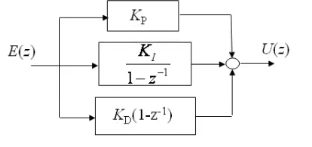
\includegraphics[width=9cm,height=4cm]{img/5_2.png}
	\caption{模拟PID控制器框图}
\end{figure}

模拟PID传递函数为:
$\frac{U(s)}{E(s)}=K_p(1+\frac{1}{T_Is}+T_Ds)$
\begin{figure}[htbp]
	\centering
	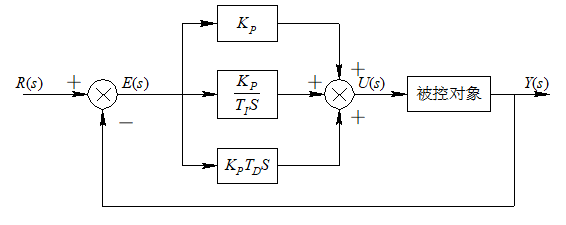
\includegraphics[width=10cm,height=4cm]{img/5_3.png}
	\caption{离散PID控制框图}
\end{figure}

既然离散PID控制器是后向差分得到的,能否将后向差分的公式$s=\frac{1-z^{-1}}{T}$带入模拟PID传递函数中,进行离散化?答案是可以的,求出来的结果与我们上述求得的完全相同
\subsubsection{增量式PID算法} 
所谓增量,就是求在前后两个采样周期之间数值增加了多少,那么就有:
$$
\Delta u(k)=u(k)-u(k-1)=
$$
$$
K_p[e(k)-e(k-1)]+K_I
e(k)+K_D[e(k)-2e(k-1)+e(k-2)]
$$
可以看到当前的增量值与三个采样周期的采样值有关,我们整理一下就有:
\begin{equation}
	\begin{aligned}
		\Delta u(k)&=a_0e(k)-a_1e(k-1)+a_2(k-2)\\ \notag
		a_0&=K_p(1+\frac{T}{T_I}+\frac{T_D}{T})\\ \notag
		a_1&=K_p(1+2\frac{T_D}{T})\\ \notag
		a_2&=K_p\frac{T_D}{T} \notag
	\end{aligned}
\end{equation}
所谓增量式,即是我当前应该在上一个基础上增加多少,那么就有:
$$
u(k)=\Delta u(k)+u(k-1)
$$
即增加上述过程中我们求出的$\Delta u(t)$
\subsubsection{控制结构图} 
对于上述两种算法,他们控制的结构图如下:
\begin{figure}[htbp]
	\centering
	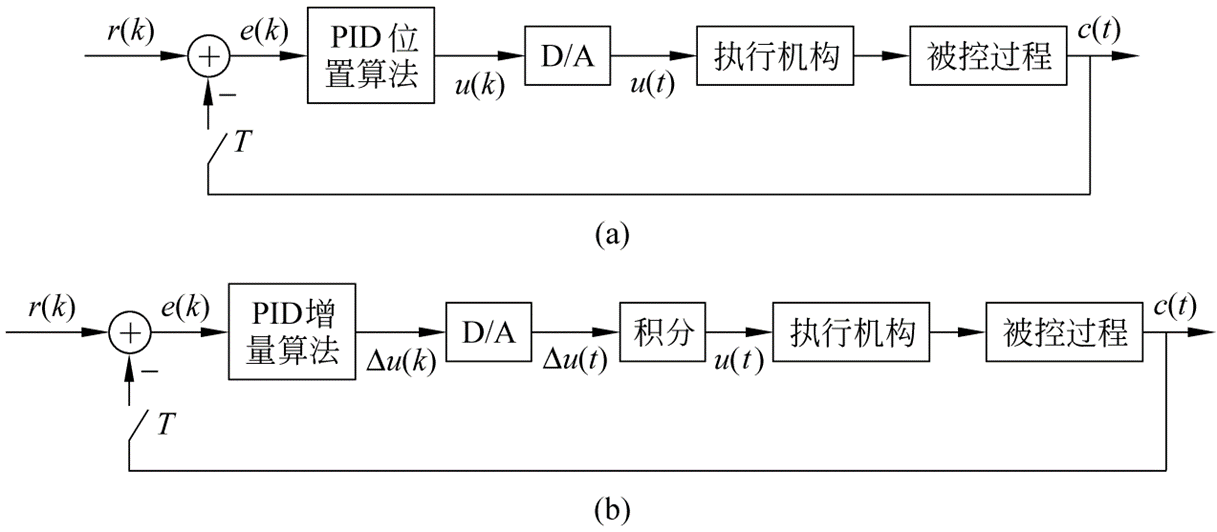
\includegraphics[width=11cm,height=4cm]{img/5_4.png}
	\caption{位置式PID与增量式PID}
\end{figure}



\subsection{PID算法的改进} 
\subsubsection{抑制积分饱和的PID算法}
在实际应用中,比如我电机的转速,阀门的开关都有一个最大值或最小值,即存在一个范围,我们控制的输出量不能超过这个范围,一旦超出限制范围,则实际执行的控制量就不再是计算值,而是系统执行机构的饱和临界值,从而引起不希望的效应
这种情况主要是由于积分项的存在,引起了PID运算的“饱和”,因此将它称为“积分饱和”,为了抑制积分饱和,他有以下几种方法:

1. 积分分离法
核心思想就是误差$e(k)$达到某个限制范围后,不让PID的积分项进行运算。
$$
u(k)=K_pe(k)+K_LK_I\sum^{k}_{j=0}e(j)+K_D[e(k)-e(k-1)]
$$
这个式子于上述得到的位置式PID仅差一个$K_L$,$K_L$称逻辑系数,当误差量$e(k)$小于某个值时,$K_L=1$,相当于有积分;$e(k)$大于某个值时,$K_L=0$,相当于没有积分。

2. 遇限削弱积分法
控制量(就是我的输出)进入饱和区间时,只执行削弱积分项累加,而不执行增大积分项的累加,即即计算$u(k)$时,先判断$u(k-1)$是否超过限制范围,若已超过$u_{max}$,则只累计负偏差;若小于$u_{min}$,则只累计正偏差,这种方法也可以避免控制量长期停留在饱和区。

3. 饱和停止积分法
与积分分离法类似,只不过这里是当输出量$u(k)$达到某个阈值时,不进行积分,达不到这个阈值时,进行积分计算。

注意:这三种方法都是有绝对值的,是一个范围,即$|u(k)或e(k)|<\epsilon$。

4. 积分限幅法
当积分项输出达到控制输出限幅值,停止积分项的值,积分项的值取前一时刻的值。
\subsubsection{干扰抑制PID算法(四点中心差分法)} 
这种算法是在$\frac{U(s)}{E(s)}=K_p(1+\frac{1}{T_1s}+T_Ds)$基础上,将微分项进行变化,然后再进行后向差分:
\begin{figure}[htbp]
	\centering
	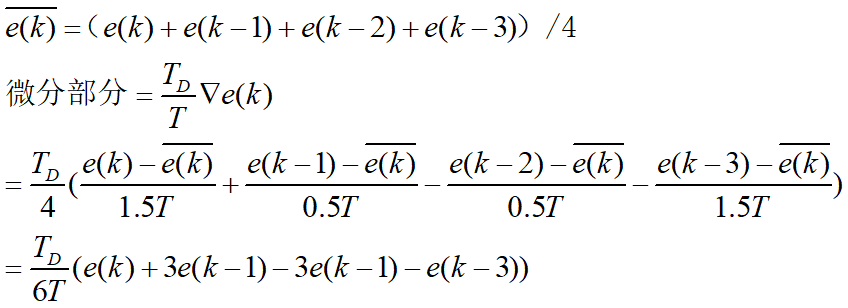
\includegraphics[width=8.48cm,height=3.08cm]{img/5_6.png}
\end{figure}
可以看到,之所以叫四点中心差分,本质上就是对四个采样值求平均数,利用这个平均数进行差分
那么,得到的位置式和增量式PID如下:
\begin{figure}[htbp]
	\centering
	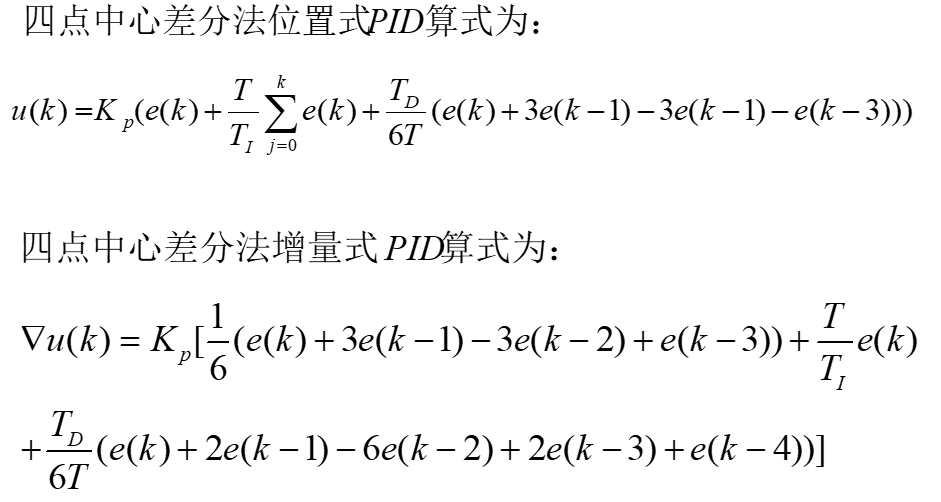
\includegraphics[width=9.4cm,height=5cm]{img/5_7.png}
\end{figure}
\subsubsection{PID算法中微分项的改进(不完全微分的PID算法)} 
在标准PID算法中,当有阶跃信号输入时,微分项输出急剧增加,控制系统很容易产生振荡,这种就是微分项造成的,我们需要对微分项进行改进。

\textbf{算法一}

其基本思想是仿照模拟调节器的实际微分调节器,加入惯性环节,以克服完全微分的缺点,根据惯性环节的位置此算法有两种结构。一种是将惯性环节加到微分上,另一种是将惯性环节加到最后面 。

那么他的控制规律如下:
$$
G'(s)=\frac{K_p}{1+T_fs}(1+\frac{1}{T_is}+T_Ds)
$$
\begin{figure}[htbp]
	\centering
	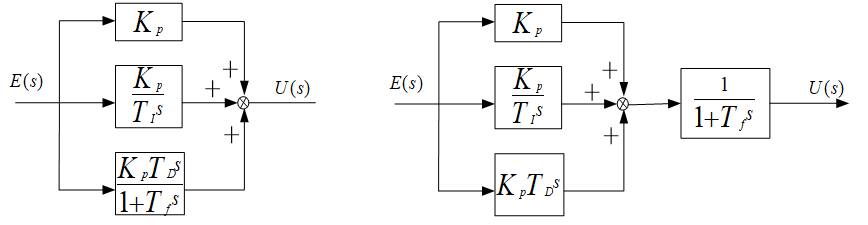
\includegraphics[width=12cm,height=3.5cm]{img/5_8.png}
	\caption{对微分进行改进后结构图}
\end{figure}

\textbf{算法二}

微分先行PID控制算法,其特点是只对输出量(也就是误差量$e(t)$)进行微分,而对输入量$u(t)$不作微分。

微分环节用$\frac{T_2s+1}{\sigma T_2s+1}$代替,那么他的控制规律如下:
$$
G'(s)=\frac{T_2s+1}{\sigma T_2s+1}K_1(1+\frac{1}{T_is})
$$

\begin{figure}[htbp]
	\centering
	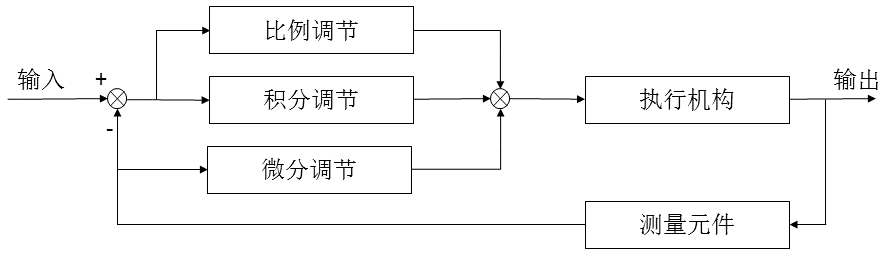
\includegraphics[width=8.8cm,height=2.5cm]{img/5_9.png}
	\caption{对微分进行改进后结构图}
\end{figure}

按后向差分带入特定式子进行离散化,有:
\begin{figure}[htbp]
	\centering
	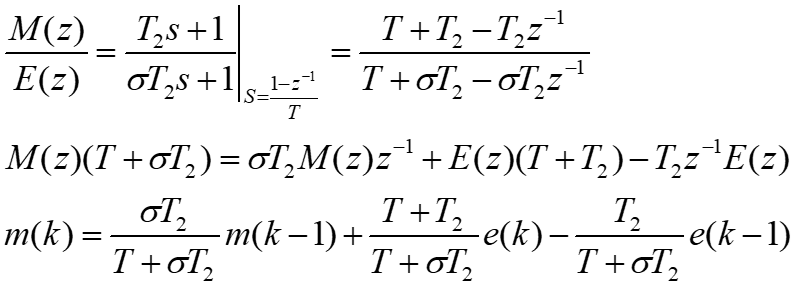
\includegraphics[width=8cm,height=2.9cm]{img/5_10.png}
\end{figure}
\newpage
\section{直接设计法}
计算机控制系统的直接设计法,是先将被控对象和保持器组成的连续部分离散化,然后应用离散控制理论的方法进行分析和综合,直接设计出满足控制指标的离散控制器,用计算机来实现。

对于没有纯滞后环节的系统来说,采用最少拍控制系统进行设计。

对于带有纯滞后环节的系统来说,采用史密斯预估器与大林算法。
带纯滞后环节系统是含滞后环节$e^{-\tau s}$的,若系统包含滞后环节,则用最少拍系统设计效果并不是很好,这里就要用到史密斯预估器与大林算法
\subsection{最少拍设计法}
最少拍设计,是指系统在典型输入信号(阶跃、速度、加速度信号)作用下,经过最少拍(有限拍),使系统输出的稳态误差为零,一般用最少拍来进行设计时,系统是不包含滞后环节的。

定义:最小拍控制为时间最优控制,即闭环控制系统在最少的采样周期内达到稳定,且在\textbf{采样点上}的输出能够准确地跟踪输入信号,不存在稳态误差。

既然是在采样点上能够准确跟踪输入信号,那么不在采样点上呢?
此时,我们可以分为两种情况:

1.有波纹:对任意两次采样时刻间的输出不提任何要求,中间可以随便震荡,只保证系统输出在采样点上误差为0,而采样点之间不保证误差为0。

2. 无波纹:采样点上及采样点间均能保证误差为0。

\noindent 一般,我们用最少拍设计得到的整个系统是如下图所示:
\begin{figure}[htbp]
	\centering
	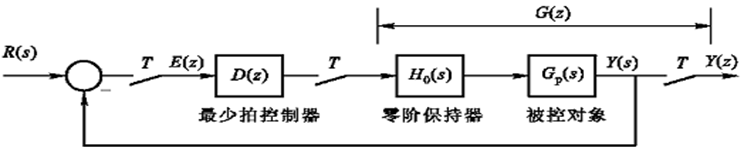
\includegraphics[width=14cm,height=3.2cm]{img/6_1.png}
	\caption{控制框图}
\end{figure}
\noindent 我们为了保证设计简单,一般假设满足以下条件:

\noindent 1. $G(Z)$在单位圆上和圆外无极点,其中$(1,0j)$除外

\noindent 2. $G(Z)$在单位圆上和圆外无零点

\noindent 3. $H_0(Z)$不含纯滞后环节

$G(z)$就是我们前面介绍的广义脉冲传递函数,直接用前面的结论做z变换:
$$
G(z)=\frac{z-1}{z}\mathcal Z[\frac{G_p(s)}{s}] = 1-z^{-1}\mathcal Z[\frac{G_p(s)}{s}]
$$

\textbf{最少拍系统设计详见附录}
\subsubsection{阻尼因子法}
我们在最小拍控制系统设计的基础上,通过在系统的闭环脉冲传递函数中,引入附加的极点因子,又称为阻尼因子;添加阻尼因子后,系统过渡过程时间增加,但整个系统的输出响应比较平稳,对不同输入信号的适应性有所改善。

那么根据上述描述,我们添加阻尼因子后的闭环传递函数$\varPhi_w(z)$为:
$$
1-\varPhi_w(z)=\frac{1-\varPhi(z)}{1-cz^{-1}}
$$
实际上,就是用$\varPhi_w(z)$替代了原来的$\varPhi(z)$,在后续算输出$Y(z)$的时候就用$\varPhi_w(z)$来计算。为了满足系统的稳定性与没有震荡的要求,应取$0<c<1$,通常我们取$c=0.5$
\subsection{史密斯预估器}
假定被控对象传递函数为:
$$
G_p(s)=G_0(s)e^{-\tau s}
$$
其中$\tau$为采样周期的\textbf{整数倍},$\tau=nT$
一般情况下,我们被控对象前面是要接零阶保持器的,我们带入零阶保持器$H_0$,经过z变换为:
$$
G(z)=z^{-n}H_0G_0(z)=z^{-n}G'(z)
$$

我们控制器仍然用$D(z)$表示,那么有:
\begin{figure}[htbp]
	\centering
	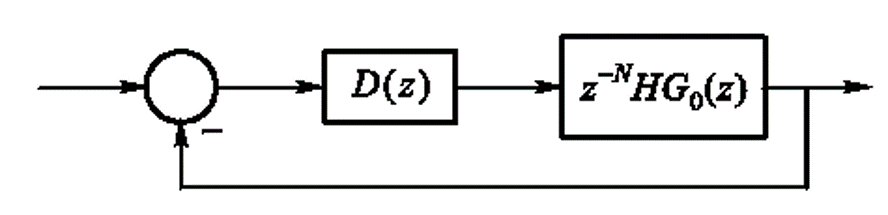
\includegraphics[width=8.88cm,height=2.15cm]{img/6_4.png}
	\caption{控制框图1}
\end{figure}

$$
\varPhi(z)=\frac{D(z)z^{-n}G'(z)}{1+{D(z)z^{-n}G'(z)}}
$$
闭环函数分母存在纯滞后环节,这是我们不想要的,因此我们的目标就是对这个闭环环节进行改造,让他的分母不再包含延迟环节。所以我们假设,将这个过程改成没有延迟环节的理想闭环系统,在其输出加上个延迟环节。
\begin{figure}[htbp]
	\centering
	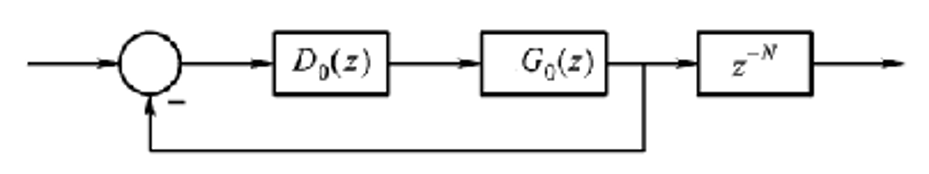
\includegraphics[width=9.29cm,height=1.74cm]{img/6_5.png}
	\caption{控制框图2}
\end{figure}
该理想系统里面,在闭环反馈的回路里已经不包含延时环节了,但由于系统的因果性限制,纯延时特性无法完全消除。

我们将二者的闭环传递函数相等,那么就可求出$D(z)$,即为史密斯预估器:
$$
D(z)=\frac{D_0(z)}{1+(1-z^{-n})D(z)G'(z)}
$$
史密斯预估器没法消除延时,但是可以使闭环系统部分不受时延影响,从而保证闭环特性的稳定和动态性能。

史密斯预估器实际上是引入了一个与被控对象并联的补偿器$(1-z^{-N})G_0(z)$,使得补偿以后的等效对象不包含纯滞后特性,为$G_0(z)$,通常情况下$D_0(z)$为PID控制器
\begin{figure}[htbp]
	\centering
	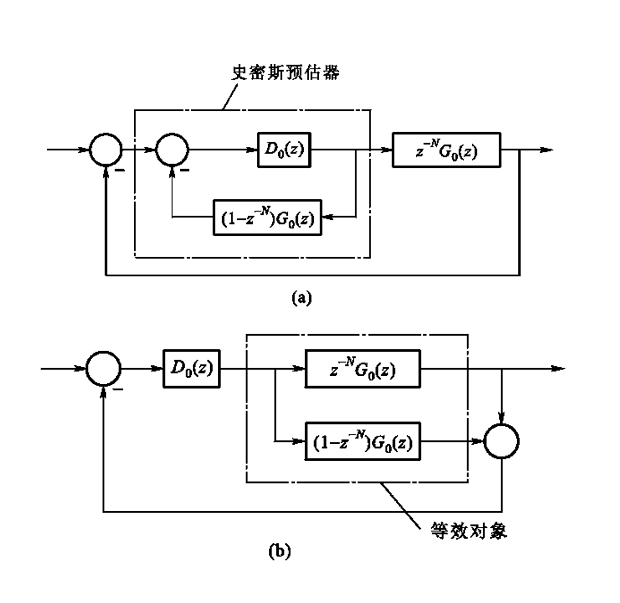
\includegraphics[width=12.4cm,height=12.06cm]{img/6_12.png}
	\caption{史密斯预估器等效图}
\end{figure}

\subsection{大林算法}
如果对系统的要求是无超调量或超调量很小,并且允许有较长的调节时间,则大林算法的控制效果往往比PID等控制算法具有更好的效果,同时大林算法也是适用于带纯滞后环节的。

我们假设带有滞后环节的控制对象可用带有滞后环节的一二阶惯性环节来表示,我们将器接入零阶保持器,然后用z变换:

\noindent 一阶惯性环节:
\begin{equation}
	\begin{aligned}
		G(z)&=\mathcal Z[\frac{1-e^{-Ts}}{s}\frac{K_pe^{-Ts}}{T_1s+1}]\\ \notag
		&=K_pz^{-(N+1)}\frac{1-e^{-\frac{T}{T_1}}}{1-e^{-\frac{T}{T_1}}z^{-1}} \notag
	\end{aligned}
\end{equation}

\noindent 二阶惯性环节:

\begin{equation}
	\begin{aligned}
		G(z)&=\mathcal Z[\frac{1-e^{-Ts}}{s}\frac{K_pe^{-Ts}}{(T_1s+1)(T_2s+1)}]\\ \notag
		&=K_pz^{-(N+1)}\frac{(c_1+c_2z^{-1})}{(1-e^{-\frac{T}{T_1}}z^{-1})(1-e^{-\frac{T}{T_2}}z^{-1})} \notag\\
	c_1&=1+\frac{1}{T_2-T_1}(T_1e^{-\frac{T}{T_1}}-T_2e^{-\frac{T}{T_2}})\notag \\ 
	c_2&=e^{-T(\frac{1}{T_1}+\frac{1}{T_2})}+\frac{1}{T_2-T_1}(T_1e^{\frac{T}{T_2}}-T_2e^{\frac{T}{T_1}})
\end{aligned}
\end{equation}
即你的被控对象如果是一阶的就用上式的一阶惯性环节来算,要是二阶的就用上式二阶惯性环节来算。

在大林算法中,无论你是一阶还是二阶,我最终的闭环传递函数都是以下形式:
$$
\varPhi(s)=\frac{1}{T_cs+1}e^{-\tau s}
$$
$\tau$与被控对象中$\tau$的相同($\tau=NT$),$T_c$为理想闭环系统的一阶惯性时间常数,该常数通过给定的设计目标来求得(设计)。
用零阶保持器法(加入零阶保持器然后进行z变换)。进行离散化,就有:
\begin{equation}
	\begin{aligned}
		G(z)&=\mathcal Z[\frac{1-e^{-Ts}}{s}\frac{e^{-\tau s}}{T_cs+1}]\\ \notag
		&=z^{-(N+1)}\frac{1-e^{-\frac{T}{T_c}}}{1-e^{-\frac{T}{T_c}}z^{-1}} \notag
	\end{aligned}
\end{equation}

\noindent 根据$D(z)=\frac{\varPhi(z)}{\varPhi_e(z)G(z)}=\frac{1}{G(z)}\frac{\varPhi(z)}{1-\varPhi(z)}$,我们可以求出$D(z)$,那么有:

\noindent 一阶惯性环节:
$$
D(z)=\frac{(1-e^{-\frac{T}{T_1}}z^{-1})(1-e^{-\frac{T}{T_c}})}{K_p(1-e^{-\frac{T}{T_1}})[1-e^{-\frac{T}{T_c}}z^{-1}-(1-e^{-\frac{T}{T_c}})z^{-N+1}]}
$$

\noindent 二阶惯性环节:
$$
D(z)=\frac{(1-e^{-\frac{T}{T_c}})(1-e^{-\frac{T}{T_1}}z^{-1})(1-e^{-\frac{T}{T_2}}z^{-1})}{K_p(c_1+c_2z^{-1})[1-e^{-\frac{T}{T_c}}z^{-1}-(1-e^{-\frac{T}{T_c}})z^{-N-1}]}
$$
\subsubsection{振铃现象}
在大林算法中,会出现振铃现象,如下图所示,一种类似于边震荡边收敛,如图所示:
\begin{figure}[htbp]
	\centering
	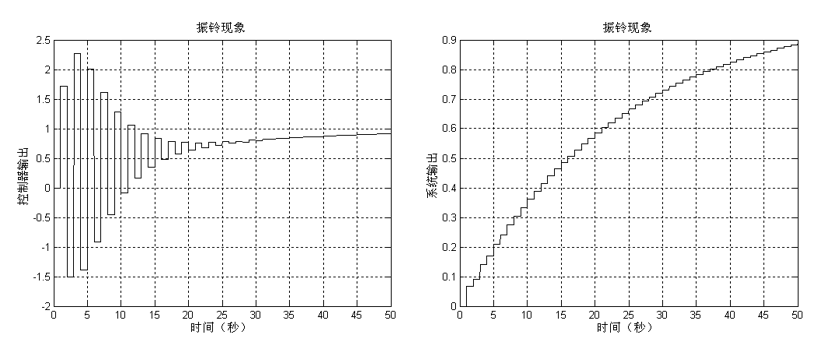
\includegraphics[width=12cm,height=5cm]{img/6_11.png}
	\caption{振铃现象}
\end{figure}

对于一阶惯性环节来说,是不存在这种现象的,只有二阶惯性环节才出现这种现象,出现这种现象出现的原因是$D(z)$存在靠近$z=-1$的极点,对此我们有两种改进方法:

\noindent 1. 选择合适的采样周期$T$及系统闭环时间常数$T_c$,使得数字控制器的输出避免产生强烈的振铃现象
我们通常用$RA$代表振铃强弱,它的定义为:
$$
RA=\frac{c_2}{c_1}-e^{-\frac{T}{T_c}}+e^{-\frac{T}{T_1}}+e^{-\frac{T}{T_2}}
$$
如果给定设计目标的$RA$,那么就可以根据上述式子调节$T$、$T_c$,以满足设计目标。

\noindent 2. 找出$D(z)$中引起振铃现象的因子,这个因子就是$z=-1$附近的极点,然后令其中的$z=1$。根据终值定理,这样处理不影响输出量的稳态值,但是会影响其动态性能指标。
例如$D(z)=\frac{1}{(1+0.995z^{-1})(1-0.795z^{-1})(1-0.765z^{-1})}$,为了消除振铃,那么就变为$D(z)=\frac{1}{1.995(1-0.795z^{-1})(1-0.765z^{-1})}$。
\section{状态空间设计法}
状态空间是现代控制原理的内容,他相当于在古典控制理论的基础上引入了状态变量,同时又可以解决多输入多输出的问题。首先,我们先介绍状态空间方程。
\subsection{状态空间方程}
在连续系统中,状态空间描述如下所式:
$$
\dot{x}(t)=A_cx(t)+B_cu(t)
$$
$$
y(t)=C_cx(t)+D_cu(t)\\
$$
$x(t)$称为状态变量,$u(t)$称为输入变量,$y(t)$称输出变量。

\noindent 第一行,我们称为状态方程,第二行,我们称为输出方程,二者和在一起称为状态空间描述又称动态方程。

自然的,在离散系统中微分方程变成差分方程,那么离散系统中状态空间描述如下:
$$
x(k+1)=Ax(k)+Bu(k)
$$
$$
y(t)=Cx(k)+Du(k)
$$
注意:为了简便起见,我们上述方程省略了了$T$,实际上$k+1\to(k+1)T$,以此类推。
\noindent 二者之间系数有如下的关系:
$$
A=e^{A_cT}\quad B=\int_0^Te^{A_cT}B_cdt\quad C=C_c\quad D=D_c
$$
\begin{table}[!ht]
	\centering
	\begin{tabular}{|l|l|}
		\hline
		x & $n$维状态矢量 \\ \hline
		u & $r$维输入矢量 \\ \hline
		y & $m$维输出矢量 \\ \hline
		A & $n\times n$系统矩阵 \\ \hline
		B & $n\times r$输入矩阵 \\ \hline
		C & $m\times n$输出矩阵 \\ \hline
		D & $m\times r$直接传递矩阵 \\ \hline
	\end{tabular}
\end{table}
对应离散系统,结构图如图所示:
\begin{figure}[htbp]
	\centering
	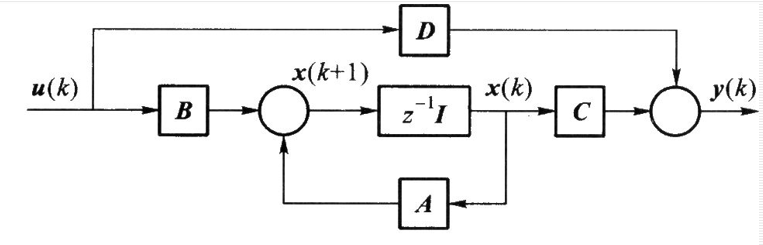
\includegraphics[width=10cm,height=3.5cm]{img/7_2.png}
	\caption{用状态空间方程描述的开环系统结构图}
\end{figure}
\subsubsection{求状态空间方程}
\noindent \textbf{方法一}:给你连续系统空间描述,利用下方系数矩阵关系求解。

$$
\left\{  
\begin{array}{lr}  
	\dot{x}(t)=A_cx(t)+B_cu(t)\\
	y(t)=C_cx(t)+D_cu(t)\\   
\end{array}      
\right.  
\Longrightarrow
\left\{  
\begin{array}{lr}  
	x(k+1)=Ax(k)+Bu(k)\\
	y(t)=Cx(k)+Du(k)\\  
\end{array}      
\right. \\
$$
$$
A=e^{A_cT}\quad B=\int_0^Te^{A_cT}B_cdt\quad C=C_c\quad D=D_c
$$
\textbf{方法二}:给定差分方程,利用如下关系求。
\begin{figure}[htbp]
	\centering
	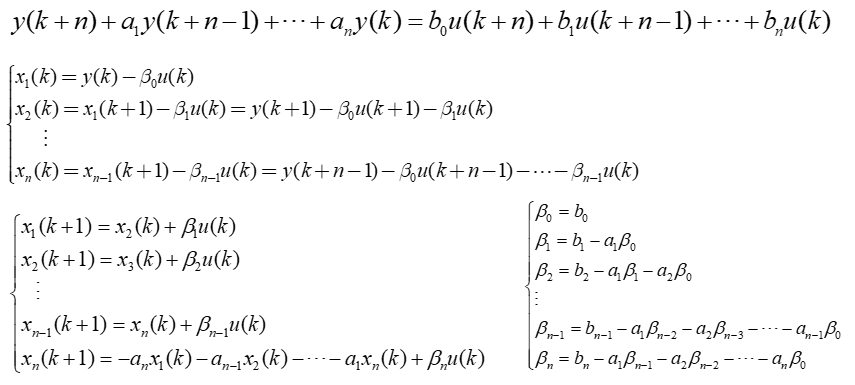
\includegraphics[width=16cm,height=8cm]{img/10_1.png}
\end{figure}
\begin{figure}[htbp]
	\centering
	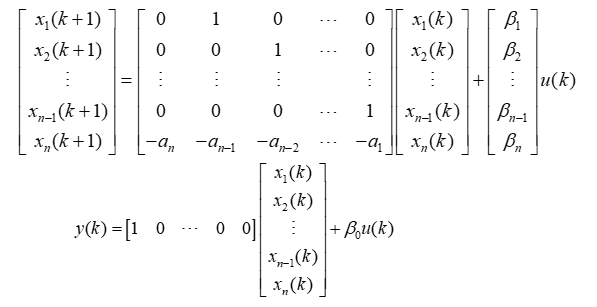
\includegraphics[width=16cm,height=8cm]{img/10_2.png}
\end{figure}
\newpage 
若是为单输入系统,则更加简单:
\begin{figure}[htbp]
	\centering
	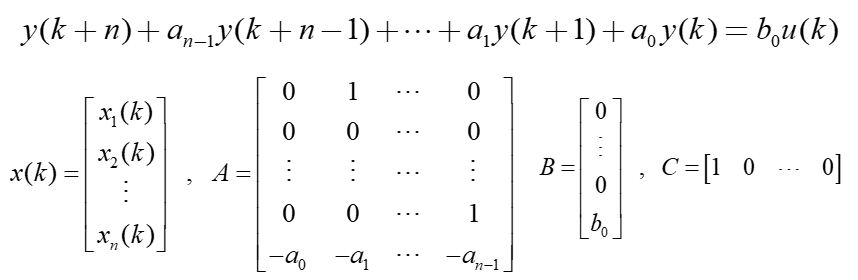
\includegraphics[width=17cm,height=5.6cm]{img/10_3.png}
\end{figure}

\subsubsection{求解状态空间方程}
此处我们默认给定系统是线性定常系统,即微分方程中各项系数都是与时间无关的常数,则称为定常系统,该类系统只要输入信号的形式不变,在不同时间输入下的输出响应形式是相同的。

我们列出了状态空间方程的目的是要求出输出的脉冲序列,那么有:

\noindent \textbf{方法一:}令$k=0,1,2···$带入,我们可得以下规律,相当于得到一个数值解:

\begin{figure}[htbp]
	\centering
	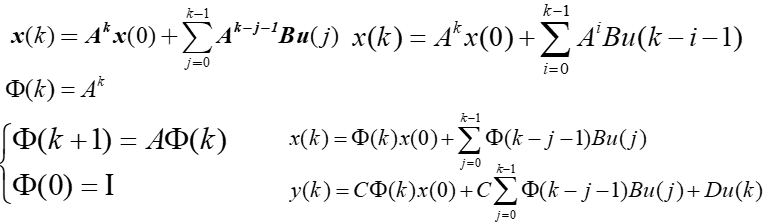
\includegraphics[width=14cm,height=4.4cm]{img/10_4.png}
\end{figure}
那么根据此规律我可以求解出任意时刻的状态空间方程。

\noindent \textbf{方法二:}利用z变换求解,实际上我们有如下规律:
$$
x(k)=\mathcal Z^{-1}[(zI-A)^{-1}z]x(0)+\mathcal Z^{-1}[(zI-A)^{-1}BU(z)]
$$
$$
y(k)=\mathcal Z^{-1}[[C(zI-A)^{-1}B+D]U(z)]
$$
此时我们可以得到解析解。
\subsubsection{能控性与能观性} 

\noindent \textbf{线性定常离散系统的能控性}

能控性,本质是在有限时间内,控制作用能否使系统从初始状态转移到要求的状态,对于线性定常离散系统状态方程:
$$
x(k+1) = Ax(k)+Bu(k)
$$
如果存在控制向量序列$u(0),u(1),\cdots,u(i-1)$,使系统从第0步的状态向量开始,在第i步到达零状态,即$x(i)=0$,那么就称此系统是能控的;如果对每一个k,系统的所有状态都是能控的,则称系统是状态完全能控的,简称能控。

判断条件:
$$
rankW_c=rank
\left[
\begin{matrix}
	B&&AB&&\cdots&&A^{n-2}B&&A^{n-1}B
\end{matrix}
\right]=n\Leftrightarrow \mbox{能控}
$$
\textbf{线性定常离散系统的能观性}

能观性,本质是在有限时间内,能够通过对系统输出的测定来估计系统的初始状态,对于线性定常离散系统状态空间描述为:
$$
x(k+1)=Ax(k)+Bu(k)\\
y(t)=Cx(k)+Du(k)\\
$$
在已知输入控制向量序列$u(0),u(1),\cdots,u(n-1)$的情况下,如果能根据有限个采样号$y(0),y(1),\cdots,y(n-1)$,确定出系统的初始状态$x_0$,则系统是状态完全能观测的,简称能观测。

判断条件:
$$
rankW_0=rank
\left[
\begin{matrix}
	C&&CA&&\cdots&&CA^{n-2}&&CA^{n-1}
\end{matrix}
\right]^T=n\Leftrightarrow \mbox{能观}
$$

\noindent \textbf{输出能控性}

判断条件:
$$rank
\left[
\begin{matrix}
	D&&CB&&\cdots&&CA^{q-1}B
\end{matrix}
\right]=m\Leftrightarrow \mbox{能控}
$$
注意:系统的状态能控性和输出能控性是两个不同的概念,二者之间没有什么必然的联系。

\subsection{状态反馈设计法}
基于状态反馈的极点配置的主要思想是,将系统的\textbf{所有}状态变量信息通过反馈增益矩阵反馈到输入端与参考输入相作用,其结果作为受控系统的控制输入。

通过对状态反馈矩阵的选择,使闭环系统的极点设置在所期望的位置上, 
采用状态反馈任意配置闭环系统极点的充分必要条件是系统状态\textbf{完全能控}。

\begin{figure}[htbp]
	\centering
	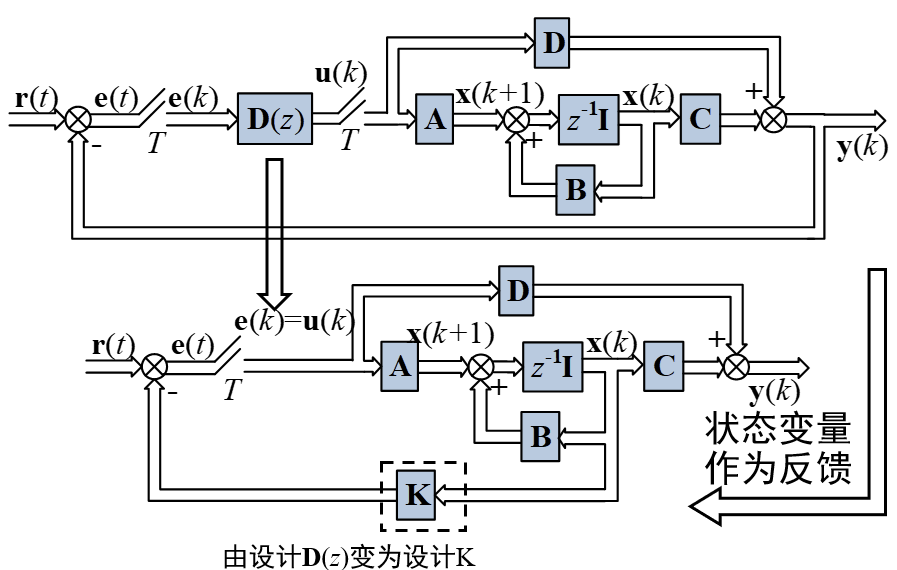
\includegraphics[width=8.9cm,height=5.9cm]{img/8_1.png}
	\caption{状态反馈设计图}
\end{figure}
\newpage
\subsubsection{状态反馈控制系统}
\begin{figure}[htbp]
	\centering
	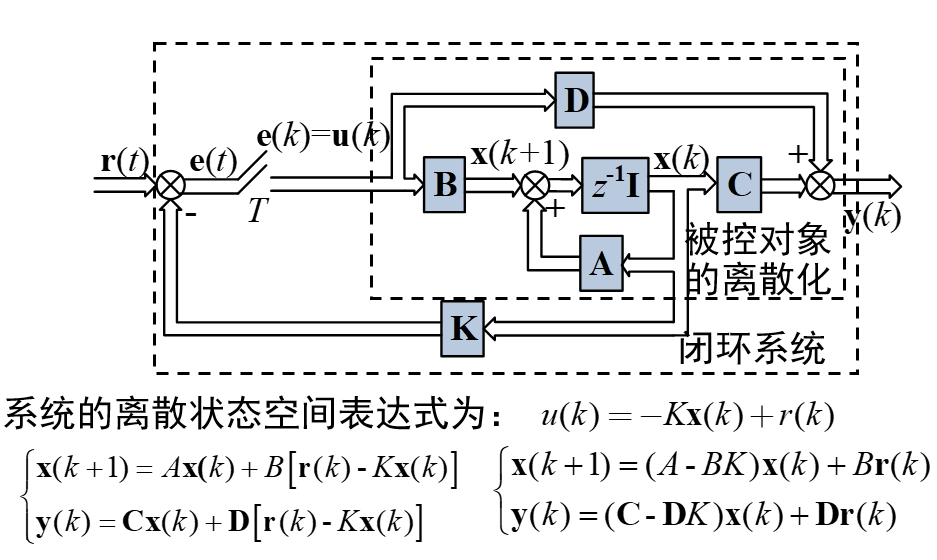
\includegraphics[width=9.3cm,height=6.8cm]{img/8_2.png}
\end{figure}
\noindent \textbf{性质:}

\noindent 1. 加入状态反馈后,不改变系统的可控性。

\noindent 2. 加入状态反馈后,闭环系统可能失去能观性。

\subsubsection{闭环Z特征方程}
\noindent 状态反馈控制系统的状态方程为:
$$
x(k+1)=(A-BK)x(k)+Br(k)
$$
左右同时进行z变换,有:
$$
zX(z)-zX(0)=(A-Bk)X(z)+BR(Z)
$$
$$
X(z)=(zI-A+BK)^{-1}(BR(Z)+ZX(0))
$$
我们称
$$
\Delta=|zI-A+BK|=0
$$
叫做状态反馈系统的闭环Z特征方程。
\subsubsection{状态反馈矩阵K的求法}
对于m维度输入n阶系统来说,K为$m\times n$,而n阶系统只有n个极点,所以要想通过期望的极点来确定K的全部参数是不可能的,有$m\times n-n$个元素可自由确定。

当考虑只有一个输入的n阶系统,那么k为$1\times n$,可由n个极点唯一确定,具体做法是利用系数匹配法,即:
$$
(z-z_0)(z-z_1)\cdots(z-z_n)=|zI-A+BK|
$$
其中$z_0,z_1\cdots z_n$为\textbf{闭环系统}期望的极点。
\subsection{输出反馈设计法}
输出反馈就是将系统的输出量经过一定的比例缩放后反馈到输入端与参考输入相作用,其结果作为受控系统的控制输入。
\begin{figure}[htbp]
	\centering
	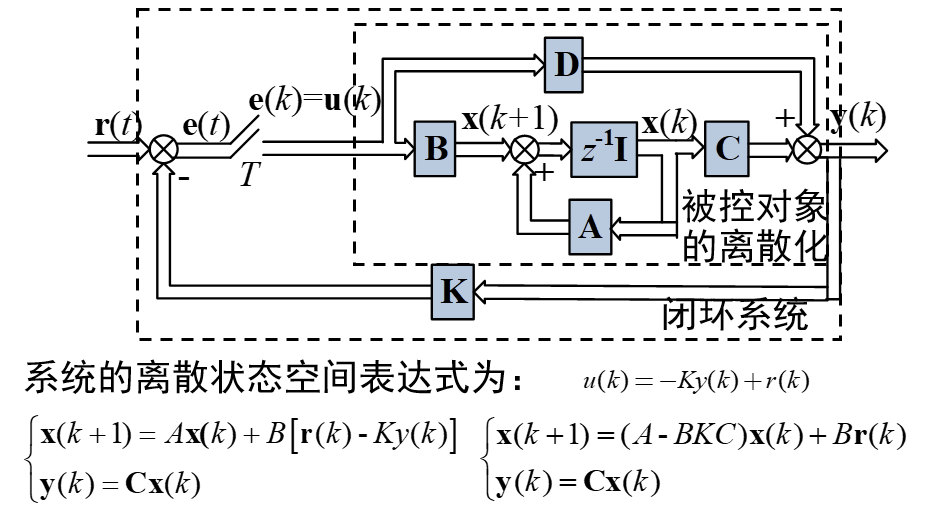
\includegraphics[width=9.25cm,height=5.16cm]{img/8_3.png}
\end{figure}
\subsubsection{特征方程与K矩阵求法}
\noindent 特征方程如下:
$$
\Delta=|zI-A+BKC|=0
$$
在仅考虑单输入系统条件下:
$$
(z-z_0)(z-z_1)\cdots(z-z_n)=|zI-A+BKC|
$$
其中$z_0,z_1\cdots z_n$为\textbf{闭环系统}期望的极点。
\subsection{状态观测器设计}
在前面中基于状态反馈设计中,是对系统的全状态进行反馈,但是在实际中测量系统所有的状态向量是困难的,甚至是不可能的。那么我能否想办法得到一个\textbf{预估值}来近似代替我测不到的状态向量呢?

状态观测器的主要思想是对系统进行重构,通过构建观测器,利用系统的控制变量和输出变量,得出系统状态变量的\textbf{估计值}。
\subsubsection{全维状态观测器的设计}
\begin{figure}[htbp]
	\centering
	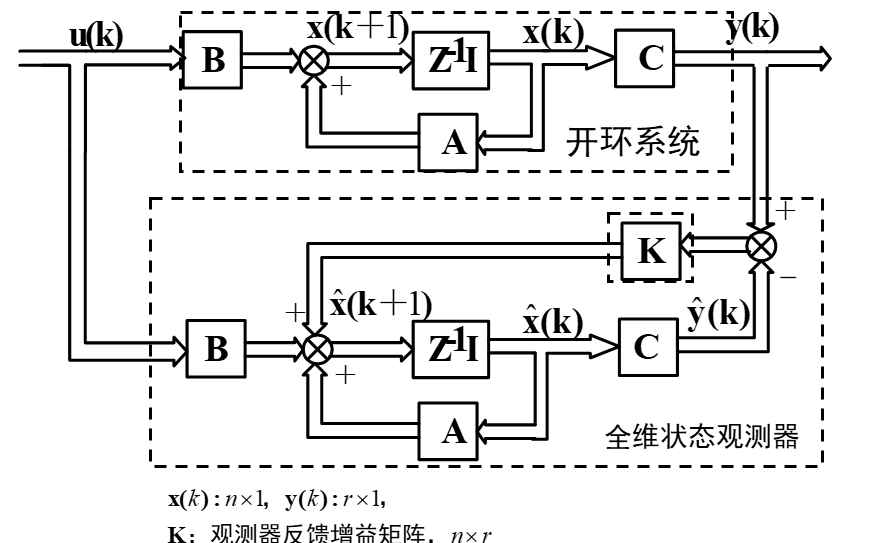
\includegraphics[width=8.7cm,height=5.4cm]{img/9_1.png}
	\caption{全维状态观测器框图}
\end{figure}
\noindent 全维状态观测器的误差方程为:
$$
\begin{aligned}
\mbox{观测误差}&=\mbox{实际值-观测值}\notag\\
\widetilde{x}(k+1)&=x(k+1)-\widehat{x}(k+1) \notag \\ 
&=Ax(k)+Bu(k)-[(A-KC)\widehat{x}(k)+Bu(K)+KCx(k)] \notag \\ 
&=(A-KC)\widetilde{x}(k)\notag
\end{aligned}
$$
经Z变换有:
$$
\widetilde{x}(z)=(zI-A+KC)^{-1}z\widetilde{x}(0)
$$
我们称观测器系统的特征方程为:
$$
\Delta=|zI-A+KC|
$$
我们设计观测器的目标是选择合适的输出误差反馈矩阵K使得状态估计误差系统的所有极点均位于z平面单位圆内,则误差可在有限拍内趋于零,即状态估计值在有限拍内可以跟踪上真实状态,且极点越靠近单位圆状态估计误差趋于零的速度越快,反之越慢。

在仅考虑单输入系统条件下:
$$
(z-z_0)(z-z_1)\cdots(z-z_n)=|zI-A+KC|
$$
其中$z_0,z_1\cdots z_n$为\textbf{观测器}期望的极点。

实际上我观测器是想得到$\widehat{x}_1(k+1)$的值,这个预测值为:
$$
\widehat{x}(k+1)=(A-KC)\widehat{x}(k)+Bu(k)+Ky(k)
$$
\subsubsection{降维状态观测器}
在系统的全部状态中,可能有一部分状态$x_2$,是可以直接在输出端获取其测量值;而另一部分$x_1$,则必须通过观测器来重构以获得估计值,在此处,我们不估计全部的状态而只估计一部分状态,那么这样的观测器就叫将为状态观测器。

那么原系统就可以分为如下几个部分:
\begin{figure}[htbp]
	\centering
	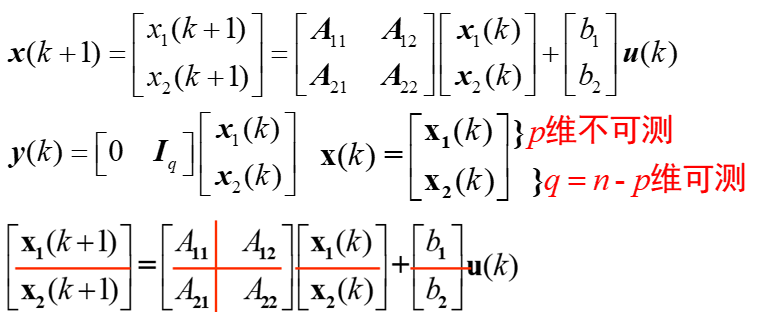
\includegraphics[width=7.6cm,height=3.2cm]{img/9_2.png}
\end{figure}
我们将第一行写出来:
$$
x_1(k+1)=A_{11}x_1(k)+A_{12}x_2(k)+b_1u(k)
$$
由于$x_2(k),x_2(k)$均是可以直接测量的,我们可以把二者当作一个整体作为新系统的$u(t)$
我们将第二行写出来,并做一个简单的变形:
$$
\begin{aligned}
x_2(k+1)&=A_{21}x_1(k)+A_{22}x_2(k)+b_2u(k)\notag \\
A_{21}x_1(k)&=x_2(k+1)-A_{22}x_2(k)-b_2u(k)\notag
\end{aligned}
$$
由于$x_2(k+1),x_2(k),u(k)$都是可以测量的,那么$A_{21}x_1(k)$相当于是新系统的$z(k)$,即设计降为状态观测器相当于设计下述系统的全维状态观测器:
$$
\begin{aligned}
x_1(k+1)&=A_{11}x_1(k)+A_{12}x_2(k)+b_1u(k)\notag \\
z(k)&=x_2(k+1)-A_{22}x_2(k)-b_2u(k)\notag
\end{aligned}
$$
同样的,误差为:
$$
\widetilde{x}_1(k+1)=x_1(k+1)-\widehat{x}_1(k+1)=(A_{11}-KA_{21})\widehat{x}_1(k)
$$

实际上我观测器是想得到$\widehat{x}_1(k+1)$的值,这个预测值为:
$$
\widehat{x}(k+1)=(A_{11}-KA_{21})\widehat{x}(k)+(A_{12}-KA_{22})x_2(k)+(b_1-Kb_2)u(k)+Kx_2(k+1)
$$

\subsection{带状态观测器的状态反馈系统}
\begin{figure}[htbp]
	\centering
	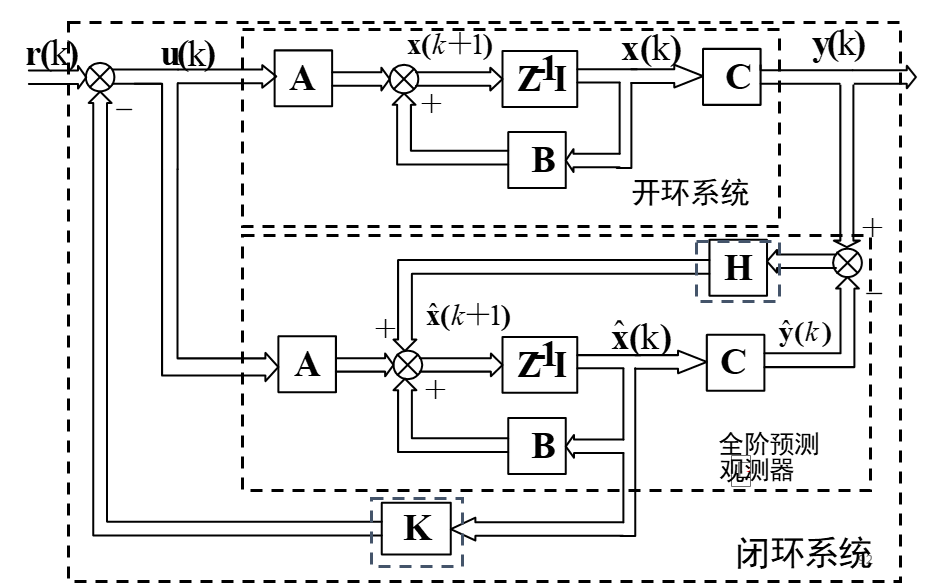
\includegraphics[width=9.3cm,height=5.8cm]{img/9_5.png}
	\caption{带状态观测器的状态反馈系统框图}
\end{figure}

\noindent 在此处,我们为了区分矩阵的区别我们称:

\noindent 1.状态反馈增益矩阵为$K$。

\noindent 2.观测器输出误差反馈矩阵为$H$。

此系统对应的特征方程为:
$$
|zI-A+BK|\cdot|zI-A+HC|=0
$$

闭环系统的2n个极点由两部分组成,一部分是按极点配置设计的控制规律给定的n个极点,称为控制极点,另一部分是按极点配置设计的状态观测器给定的n个极点,称为观测器极点。两部分相互独立,可分别设计。

分离原理:设计基于观测状态的状态反馈控制系统时,对观测器和控制器的设计是分别独立进行的,分别找到状态观测器的特征根方程和闭环系统的特征方程,根据给定的期望极点,分别得到观测器反馈增益矩阵$H$和状态反馈增益矩阵$K$。
\newpage
\chapter{附录}
\end{document}
